The most straightforward method of improving a game's performance is to simply cut some content, or lower the quality of some aspects. It consists of many small changes, that together may (hopefully) have a noticeable impact. The game should be analysed against the target platforms. Perhpas the resolution of some textures is too high for a target platform, or perhaps the game world can be reduced in scale. Unity provides a great tool for managing quality, enabling the developer to create Quality Settings profiles for the project. These can affect and overwrite certain effect specific settings, and can be freely distributed across target platforms. Texture resolution can be decreased from the original, high-quality texture, shadow and rendering improvements such as Anti Aliasing can be reduced, or disabled altogether, without impacting other platforms. A study released by the Hindawi Publishing Corporation confirms that visual quality of an image relies not only on the image itself, but is also closely tied to the characteristics of the screen displaying them. Resolution, pixel density, screen size, all influence and potentially bottleneck the quality of the image that the end-user will see. \cite{imgquality}. \\ \\
The original Space Shooter comes with full quality of all its assets. The original skybox texture has a 4k resolution, and the game world consists of 512 asteroids and 30 hostile drones, continuously firing towards the player. All special effects, such as particles, will be left as created, with visual quality as a priority. \\
One aspect to note, a traditional game development technique has already been implemented, because the other option was not only cumbersome to implement, but also highly inefficient on both development time and resources. The asteroid field consists of only 4 distinct asteroid models, slightly altered in scale by randomized deltas. Having 512 distinct asteroid models is both a daunting graphical design task, and non-scalable for increasinly big fields. As such, one useful technique is Model/Texture Sharing. With a small, yet sufficiently large pool of assets, an illusion of diversity can be created that is indistinguishably close to real diveristy during play time, but with a fraction of the resources needed.
Another quality setting that affects performance is Anti Aliasing. Because 3D objects are rendered in a game as a mesh of triangles, sometimes the shapes are rendered with jagged edges. Anti Aliasing addresses this, but through a relatively expensive computational process on the GPU. The effect however seems less severe on a smaller screen, therefore it may be useful to remove this effect altogether in the Android release of the game. As stated in the presentation attached to this article, mobile gaming is not aimed to directly compete with ``bigger'' platforms such as PC or consoles, but as an ``on the go'' option. 
High-quality shadows and reflections can also negatively influence a game's performance, and may grow unnoticed in a high-action game. The traditionally used rendering method, rasterization, already uses light maps for an approximation of realistic shadows, and as a time-tested method, an indication that perfect simulation of reality is often not necessary for an enjoyable gaming experience. Unlike the state of the art real time ray tracing technology released in August 2018 by Nvidia, rasterization is much less computationally intensive, but even so, without optimizations, a game can be quite difficult for hardware to run within acceptable parameters. \\ \\
In an attempt to optimize the game based on the previously mentioned methods, the following changes have been done to Space Shooter in an attempt to improve the performance:
\begin{enumerate}
\item{Skybox texture base resolution has been reduced to 1k, from 4k}
\item{Rendering resolution of the skybox texture has been reduced to one eighth of the base resolution}
\item{Enemy drone count has been reduced to 20, down from 30}
\item{Asteroid count has been reduced to 216, down from 512}
\item{Explosion particle count and emission rate have been greatly reduced}
\item{Anti aliasing has been completely removed}
\item{Shadows and reflections have been disabled}
\end{enumerate}
The results are quite interesting. The framerate in the unoptimized games has been quite even, except for the spikes associated with restarting a level and reinitalizing the game world to the original state. Figure 5 shows the framerates across the 5 tests pre and post optimizations for both platforms, and we can see that especially on PC (Android as well, but less so), the framerate has high fluctuations, but overall is in a higher value range than before. Table 2 shows even more details. Overall, there has been a 133.44\% improvement on PC, but the standard deviation has increased over 5 times. This indicates that there are other components of the game that would require further optimization. Looking at the Android values, they seem less impatctful when looking at the graph. With only 14.56\% improvement post optimization, the standard deviation is still significantly higher, by a magnitude greater than 3. This further enforces the hypothesis that while results are better, further optimization areas need to be found. Looking at the minimum values on the Android device, we notice that they are unchanged, at 10. This would indicate that a specific resource is extremely heavily used, and proving a main bottleneck factor.
\begin{figure}
\begin{subfigure}{0.49\textwidth}
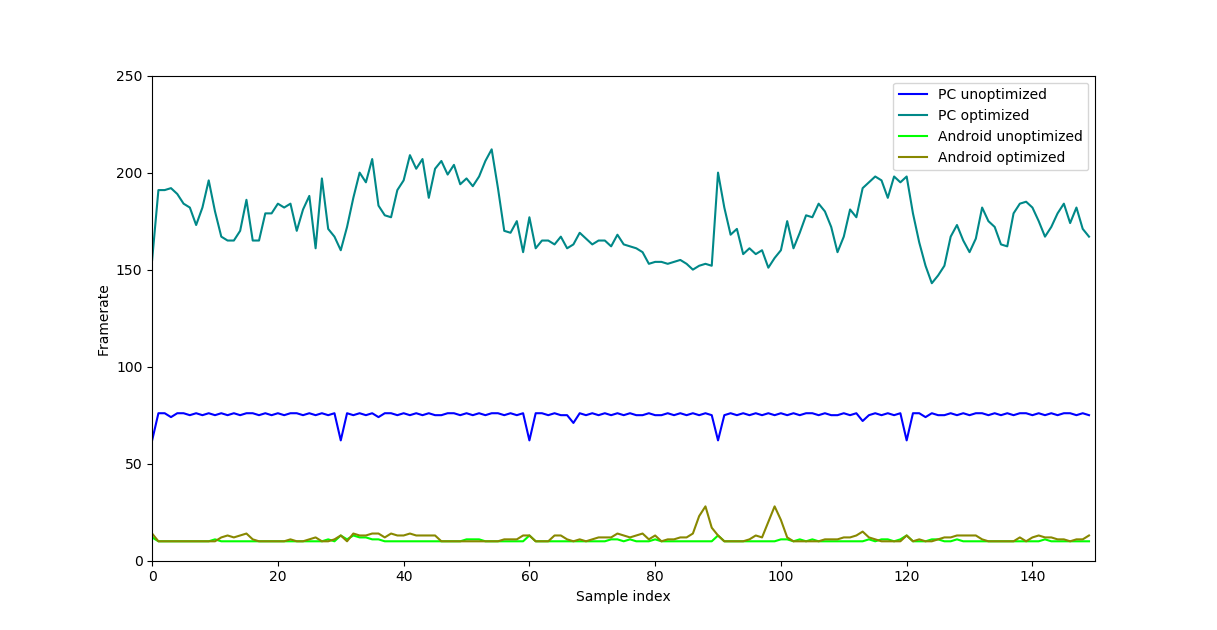
\includegraphics[width = \textwidth, height = 0.66\textwidth]{images/compromise}
\end{subfigure}
\caption{Framerate before and after optimization}
\end{figure}
\begin{table}
\caption{Optimization data}
\label{tab:conf}
\begin{minipage}{0.49\textwidth}
\begin{center}
\begin{tabular}{lllll}
Value & PC pre & PC post & Android pre & Android post \\
Mean & 75.00 & 175.08 & 10.30 & 11.82 \\
Std & 2.51 & 15.68 & 0.67 & 2.75 \\
Top 10 mean & 76.00 & 205.50 & 12.30 & 19.40 \\
Bottom 10 mean & 67.50 & 150.50 & 10.00 & 10.00 \\
Min & 62 & 143 & 10 & 10 \\
Max & 76 & 212 & 13 & 28 
\end{tabular}
\bigskip
\end{center} 
\end{minipage}
\end{table}